\chapter{数据库设计}
\section{数据库环境说明}
本聊天软件的服务器在云服务器上运行,操作系统是Ubuntu16.04,所以本系统的数据系统采用MySQL数据库系统。

\section{数据库的命名规则}
不允许单词缩写,表名是复数形式。

\section{逻辑设计}
本数据库的users和links表能满足BCNF范式,但是unreceived\_message表并不设主键,仅仅满足第一范式。
\begin{figure}[h]
	\centering
	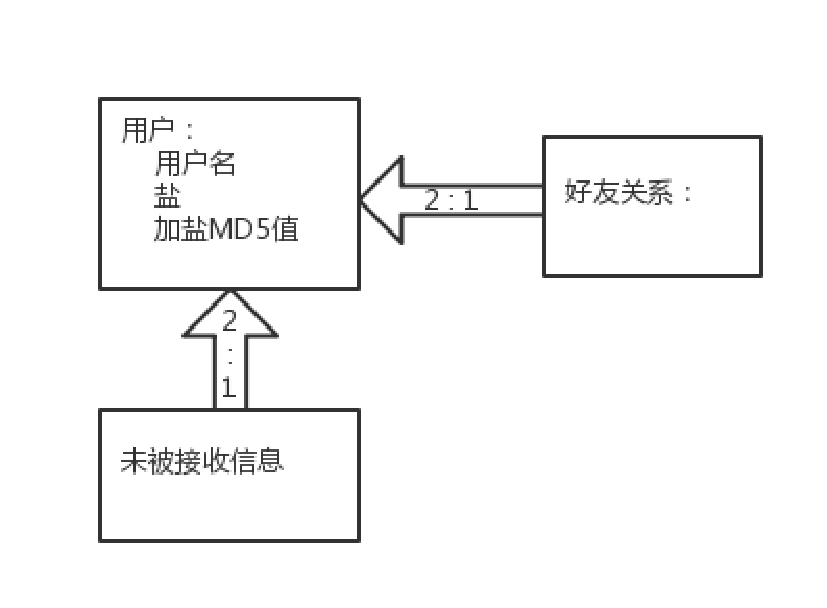
\includegraphics[width=10cm]{fig_db}
\end{figure}

\section{物理设计}
\subsection{数据库产品}
使用MySQL数据库。根据目前本软件的使用情况,一台云服务器已经可以很好地满足所有需求,所以没有采用分布式数据库。
\subsection{实体属性、类型、精度}
\subsubsection{客户数据表设计}
\begin{table}[htbp]
\centering
\caption{用户数据表Users设计} \label{tab:client-database}
\begin{tabular}{|c|c|c|c|c|}
    \hline
    字段名 & 类型 & 大小 & 说明 & 备注 \\
    \hline
    uname & varchar & 48 & 用户名 & 主键\\
    \hline
    md5 & char & 10 & 随机产生的加盐值 & ·\\
    \hline
    pw & char & 32 & 用户的登录密码加盐的MD5值 & · \\
    \hline
\end{tabular}
\note{用户数据表Users设计}
\end{table}

\subsubsection{联系人数据表设计}
\begin{table}[htbp]
\centering
\caption{联系人表Links设计} \label{tab:order-database}
\begin{tabular}{|c|c|c|c|c|}
    \hline
    字段名 & 类型 & 大小 & 说明 & 备注 \\
    \hline
    uname\_1 & varchar & 48 & 用户1 & 主键,外键,引用Users\\
    \hline
    uname\_2 & varchar & 48 & 用户2 & 主键,外键,引用Users \\
    \hline
\end{tabular}
\note{联系人表Links设计}
\end{table}
\section{安全性设计}
服务器调用数据库全部采用存储过程,不允许直接执行数据库语句,一般不会产生安全性问题。

\section{数据库管理与维护说明}
对于数据库的维护,随时对数据库中的信息加以调试和保存备份。同样需要个工作人员进行系统的分析和用户的反馈,对系统进行升级以及功能的完善。同时保证系统安全有序的运行。